% 02-main/ch2_analysis.tex

\chapter{État de l'art}
\label{chap:analysis}

Ce chapitre dresse un état de l'art des avancées récentes dans la vision par ordinateur, la cartographie du potentiel solaire et l'analyse des toitures. Il examine les différentes méthodes et technologies développées dans ces domaines, en mettant l'accent sur les approches les plus innovantes et leurs applications pratiques.

\localtableofcontents

\newpage

% -----------------------------------------------------------------------------
% -----------------------------------------------------------------------------
\section{Introduction}
\par{L'évaluation du potentiel solaire des toitures est un élément clé de la transition énergétique urbaine. Sa précision dépend directement de la qualité et de la disponibilité des données utilisées, qui peuvent provenir de différentes sources avec des niveaux de détail variables.}

\par{Les méthodologies d'évaluation du potentiel solaire s'appuient principalement sur quatre types de données :}
\begin{enumerate}
    \item Données du cadastre
    \item Modèle tridimensionnel des bâtiments et du territoire
    \item Données géomatiques
    \item Orthophotos
\end{enumerate}

\par{La deuxième partie de ce chapitre va traiter les articles scientifiques qui utilisent du machine learning pour réaliser de la segmentation de toitures.}

\par{Ensuite, une troisième partie sera dédiée aux dataset disponibles.}

\par{Une brève synthèse permettra de conclure et de justifier l'approche utilisée.}

\par{Les notions théoriques nécessaires pour la compréhension de ce chapitre se trouvent dans deux annexes. Le premier traite de  l'énergie solaire et ses applications dans l'annexe ``\nameref{chap:fondamentaux_energie}''. Le deuxième annexe ``\nameref{chap:fondamentaux_ml}'' va permettre d’avoir les bases nécessaires pour comprendre ce qu’est le machine learning, ses
limites et ses applications.}

% -----------------------------------------------------------------------------
% -----------------------------------------------------------------------------
\section{Évaluation du potentiel solaire des toitures}

% -----------------------------------------------------------------------------
\subsection{Analyse du potentiel photovoltaïque des toitures résidentielles en Andalousie}

\subsubsection{Contexte et objectifs}
\par{L'étude menée par \citeauthor{ordonez_analysis_2010} \cite{ordonez_analysis_2010} présente une analyse détaillée du potentiel de production d'énergie photovoltaïque sur les toitures résidentielles en Andalousie (Espagne). Cette région, avec une radiation solaire moyenne de 4,75 kWh/m² par jour et une superficie de 87 597 km², possède le plus fort potentiel solaire d'Europe.}

\subsubsection{Données}
\par{Les données utilisées dans cet article sont :}
\begin{itemize}
    \item Données du cadastre et les surfaces de toiture renseignées lors des autorisations de construire
    \item Orthophotos de google maps
\end{itemize}

\subsubsection{Méthodologie}
\par{La méthodologie repose sur trois volets complémentaires :}
\begin{itemize}
    \item L'analyse statistique des données du cadastre qui répartit les logements en trois types : les maisons individuelles ou jumelées, les maisons en bande, et les immeubles collectifs
    \item L'estimation des surfaces type de toit réellement utilisables pour les panneaux solaires, en prenant en compte tous les obstacles (cheminées, antennes, etc.), les zones d'ombre et les autres contraintes
    \item L'étude de l'ensoleillement moyen de la région et des performances des systèmes photovoltaïques, basée sur les caractéristiques techniques des panneaux disponibles
\end{itemize}

\subsubsection{Résultats principaux}
\par{L'analyse a permis d'identifier les potentiels suivants :}
\begin{itemize}
    \item La surface totale de toiture disponible est de 265,52 km², dont 218,52 km² (82,29\%) sont effectivement utilisables pour des installations photovoltaïques
    \item Le potentiel de production énergétique est estimé à 9,73 GWh/an pour des panneaux IS-170 et 9,38 GWh/an pour des panneaux IS-220
    \item Cette production permettrait de couvrir environ 78,89\% des besoins énergétiques du secteur résidentiel andalou, réduisant la dépendance énergétique extérieure à seulement 21,02\%
\end{itemize}

\subsubsection{Discussion et limites}
\par{Cette recherche démontre qu'il est possible d'estimer le potentiel solaire des toitures à partir de données déjà existantes, sans qu'il soit nécessaire d'investir dans l’acquisition de nouvelles données.}

\par{La méthodologie utilisée, bien que statistiquement solide, présente certaines limites. Notamment, elle s'appuie uniquement sur les données cadastrales issues des autorisations de construire et des enquêtes gouvernementales. Lors de la rédaction de cet article (2010), les auteurs se sont basés sur des données de 2000-2007. Actuellement, ils disposent de données \gls{lidar} \cite{nacional_plan_nodate} qui permettraient une évaluation plus précise et exhaustive du potentiel solaire pour l'Andalousie.}

% -----------------------------------------------------------------------------
\subsection{Cadastre solaire Genevois}

\par{Il y a une multitude d'article dédiés à l'étude du potentiel solaire, la région de Genève est l'une des régions du monde avec le plus d'articles publiés après Wuhan (Chine) \cite{drozd_evaluating_2025}. \citeauthor{thebault_large-scale_2022} \cite{thebault_large-scale_2022} vont analyser la pertinence de la pose de panneaux solaire \acrshort{pv} au niveau du \gls{grandgeneve}.}

\subsubsection{Contexte et objectifs}
\par{Le premier cadastre solaire de Genève \cite{desthieux_etude_2011} date de 2011. Il est réalisé par hepia, l'EPFL et le Politecnico di Milano, financé par les Services Industriels Genevois et le Service de l'énergie du canton (actuellement l'OCEN). Elle vise à cartographier précisément le potentiel solaire sur les toitures genevoises. Les données utilisées sont :}
\begin{itemize}
    \item Données LiDAR de 2009 (4-6 points/m$^2$)
    \item Empreinte au sol des toitures issues du modèle vecteur 3D du bâti sur le canton de 2005
    \item Données météo horaires issues de Meteonorm.
\end{itemize}
La méthodologie utilisée est la suivante :
\begin{itemize}
    \item Construction d'un modèle numérique de surface 2.5D à partir de données LiDAR et d'empreintes au sol des bâtiments
    \item Calcul de l'irradiation solaire horaire sur les toits en tenant compte des ombrages (bâti, végétation, relief), à l'aide d'un outil développé sous Matlab
    \item Production d'indicateurs et de statistiques d'irradiation par toiture dans ArcGIS
\end{itemize}
\par{Le résultat de l'étude est une couche vectorielle qui indique l'irradiation solaire pour la toiture d'un bâtiment. Le temps de calcul est d'environ 2000 h pour une seule machine.}

\par{Une deuxième phase du cadastre est effectuée en 2014 \cite{desthieux_etude_2014} qui permet d'améliorer la modélisation des toitures, le calcul de l'irradiation solaire et de réaliser certains prédimensionnements :
\begin{itemize}
    \item Estimation de production d'électricité
    \item Estimations pour le solaire thermique
    \item Indicateurs économiques
\end{itemize}}
\par{Cette mise à jour positionne le cadastre solaire comme outil d'aide à la décision. Le rendu de l'étude est constitué de plusieurs couches vectorielles. La figure \ref{fig:cadastre_solaire_2014} illustre les informations disponibles.}
\begin{figure}[H]
    \centering
    \includegraphics[width=1\linewidth]{02-main//figures/cadastre_solaire_2014.png}
    \caption{Image d'exemple avec une partie des informations disponibles par bâtiment \cite{desthieux_etude_2014}.}
    \label{fig:cadastre_solaire_2014}
\end{figure}

\par{En 2016, le cadastre a été mis à jour \cite{desthieux_solar_2018}. Les principales nouveautés sont :
\begin{itemize}
    \item L'utilisation des données LiDAR de 2013 \cite{sitg_nuages_2013}
    \item L'amélioration des algorithmes de calcul du potentiel solaire
    \item Utilisation d'un cluster (24 machines) pour réaliser les calculs (environ 900h)
\end{itemize}}

\par{Dès 2018, plusieurs mises à jour \cite{desthieux_solar_2018} sont effectuées. Les principales nouveautés sont :
\begin{itemize}
    \item Prise en compte des toitures et des façades des bâtiments pour l'évaluation du potentiel solaire
    \item Amélioration des algorithmes de calcul du modèle de ciel
    \item Réécriture du code Matlab en Java
    \item Utilisation du cloud CTI IceBOUND
    \item Expansion du cadastre solaire au Grand Genève (canton de Genève, district de Nyon, et pôle métropolitain du Genevois Français)
\end{itemize}}

\par{En 2020, l'article \cite{stendardo_gpu-enabled_2020} de \citeauthor{stendardo_gpu-enabled_2020} aborde la question de l'optimisation des calculs pour le cadastre du Grand Genève. Les auteurs proposent l'utilisation des \acrshort{gpu} pour réduire considérablement les temps de traitement. Cette amélioration répond à un défi croissant : chaque nouvelle version du cadastre intègre davantage de données et requiert des calculs plus précis, ce qui allonge inévitablement les temps d'exécution. L'optimisation du code devient donc un aspect fondamental pour la viabilité du projet.}
\begin{figure}[H]
    \centering
    \includegraphics[width=1\linewidth]{02-main//figures/cadastre_solaire_gpu.png}
    \caption{Schéma pour le calcul d'une tuile}
    \label{fig:cadastre_solaire_gpu}
\end{figure}
La Figure \ref{fig:cadastre_solaire_gpu} montre comment le traitement a été repensé pour chaque tuile de 3 x 3 km. Les parties du code Java qui pouvaient être massivement parallélisées ont été réécrites en CUDA \cite{nvidia_cuda_nodate}, ce qui permet de tirer parti des \acrshort{gpu} au lieu de s'appuyer uniquement sur les \acrshort{cpu}. Les autres parties critiques du code ont été optimisées en C++ \cite{noauthor_c_2025}. On peut voir sur la Figure \ref{fig:cadastre_solaire_gpu_evolution_temps} que cette approche a permis de réduire considérablement le temps de traitement par tuile.

\begin{figure}[H]
    \centering
    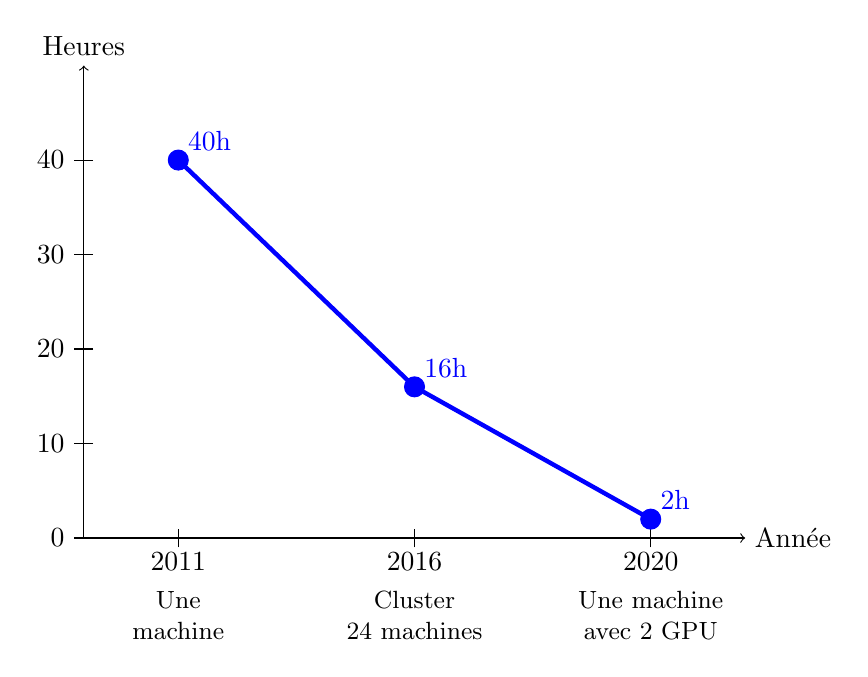
\begin{tikzpicture}[scale=1.2]
        % Axes
        \draw[->] (0,0) -- (7,0) node[right] {Année};
        \draw[->] (0,0) -- (0,5) node[above] {Heures};
        
        % Graduations - en commençant par 1 au lieu de 0
        \foreach \y in {1,2,3,4}
            \draw (0.1,\y) -- (-0.1,\y) node[left] {\y0};
        
        % Ajouter le 0 séparément
        \draw (0.1,0) -- (-0.1,0) node[left] {0};
        
        % Années
        \foreach \x/\year in {1/2011, 3.5/2016, 6/2020}
            \draw (\x,-0.1) -- (\x,0.1) node[below=5pt] {\year};
        
        % Données
        \draw[blue, ultra thick] (1,4) -- (3.5,1.6) -- (6,0.2);
        
        % Points
        \filldraw[blue] (1,4) circle (3pt) node[above right] {40h};
        \filldraw[blue] (3.5,1.6) circle (3pt) node[above right] {16h};
        \filldraw[blue] (6,0.2) circle (3pt) node[above right] {2h};
        
        % Annotations
        \node[align=center, font=\small, below] at (1,0) {\\\\Une\\machine};
        \node[align=center, font=\small, below] at (3.5,0) {\\\\Cluster\\24 machines};
        \node[align=center, font=\small, below] at (6,0) {\\\\Une machine\\avec 2 GPU};
    \end{tikzpicture}
    \caption{Évolution des temps de calcul par tuile pour le cadastre solaire (2011-2020).}
    \label{fig:cadastre_solaire_gpu_evolution_temps}
\end{figure}

\subsubsection{Données}

\subsubsection{Méthodologie}

La méthodologie \cite{desthieux_solar_2018} pour la création du cadastre suit les étapes suivantes :
\begin{itemize}
    \item Collecte des données
    \item Construction du modèle 3D
    \item Calcul des ombrages
    \item Calcul de l'irradiation solaire en chaque point des toits et façades
    \item Calcul des indicateurs et visualisation des résultats
\end{itemize}

La Figure \ref{fig:cadastre_solaire_methodologie} résume ces points.
\begin{figure}[H]
    \centering
    \includegraphics[width=1\linewidth]{02-main//figures/cadastre_solaire_methodologie.png}
    \caption{Méthodologie utilisée pour la création du cadastre solaire \cite{desthieux_solar_2018}}
    \label{fig:cadastre_solaire_methodologie}
\end{figure}

\paragraph{Collecte des données}
\par{La première étape est d'obtenir les données nécessaires ("Raw data" sur la Figure \ref{fig:cadastre_solaire_methodologie}). À partir des données LiDAR, on construit deux modèles 3D de la ville : un modèle numérique de surface (DSM) qui représente la surface supérieure des bâtiments et de la végétation, et un modèle numérique de terrain (DTM) qui représente le sol nu sans les bâtiments.}
\par{Les contours et empreintes des toits et bâtiments  sont aussi récupérés à partir de données cadastrales existantes, en 2D et 3D. Ils serviront à délimiter précisément les toits et façades.}

\paragraph{Construction du modèle 3D détaillé}
\par{La deuxième étape consiste à construire un modèle 3D détaillé de la ville ("mask inputs" sur la Figure \ref{fig:cadastre_solaire_methodologie}), qui servira de base aux calculs d'ensoleillement. Ce modèle est créé à partir des données récoltées à l'étape précédente.}
\par{Tout d'abord, le modèle numérique de surface (DSM) et le modèle numérique de terrain (DTM) sont transformés en images 3D appelées "rasters". Imaginez une grande grille recouvrant toute la ville, où chaque case de la grille (appelée "pixel") contient une valeur de hauteur. C'est exactement ce que sont le DSM et le DTM : des grandes grilles 3D où la hauteur de chaque point de la ville est enregistrée.}
\par{Ensuite, deux modèles 3D distincts sont créés : un pour les toits et un pour les façades. Pour cela, on combine le DSM obtenu à partir des données LiDAR avec les données cadastrales qui contiennent les contours des bâtiments. Cela permet d'avoir un modèle 3D, où chaque toit et chaque façade est représenté.}
\par{Pour chaque pixel du modèle 3D des toits, deux informations supplémentaires sont calculées : la pente (c'est-à-dire l'inclinaison) et l'orientation (nord, sud, est, ouest...). Ces deux paramètres sont très importants car ils influencent grandement la quantité d'énergie solaire reçue. Par exemple, un toit plat horizontal recevra plus de soleil qu'un toit très pentu orienté vers le nord.}
\par{Le modèle 3D des façades est un peu plus complexe à créer. En effet, un modèle "raster" comme celui des toits ne permet pas de bien représenter les surfaces verticales. Pour contourner ce problème, des points supplémentaires appelés "hyperpoints" sont ajoutés le long des façades (voir Figure \ref{fig:cadastre_solaire_hyperpoints}). Ils permettent de représenter chaque façade comme une série de points verticaux, sur lesquels on pourra ensuite calculer l'ensoleillement de manière précise.}
\begin{figure}[H]
    \centering
    \includegraphics[width=1\linewidth]{02-main//figures/cadastre_solaire_hyperpoints.png}
    \caption{Méthode de création des hyperpoints sur les façades \cite{desthieux_solar_2018}}
    \label{fig:cadastre_solaire_hyperpoints}
\end{figure}
\par{Finalement, on obtient un jumeau numérique très détaillé de la ville, avec un modèle 3D distinct pour les toits et les façades. Ce jumeau numérique contient toutes les informations nécessaires (hauteur, pente, orientation) pour calculer finement l'ensoleillement en tout point. Les étapes suivantes vont s'appuyer sur ce modèle pour simuler les ombres portées et calculer le potentiel solaire.}

\paragraph{Calcul des zones d'ombre}
\par{La troisième étape consiste à calculer les zones d'ombre sur les toits et les façades des bâtiments (« mask inputs » sur Figure \ref{fig:cadastre_solaire_methodologie}). Cette étape est cruciale car les zones ombragées ont un potentiel solaire significativement inférieur aux zones bien exposées au soleil.}
\par{Pour réaliser ce calcul, le jumeau numérique 3D de la ville créé précédemment est utilisé comme base. Ce modèle contient toutes les informations nécessaires sur la forme et la hauteur des bâtiments et du relief environnant. Un algorithme de simulation reproduit la course du soleil heure par heure tout au long de l'année, projetant les ombres correspondantes sur le modèle 3D.}
\par{L'ombrage représente l'un des facteurs les plus déterminants pour la performance d'une installation solaire. Pour analyser précisément son impact, trois catégories principales d'ombrages sont identifiées:}
\begin{itemize}
    \item Les ombrages proches: Causés par des éléments situés directement sur le toit comme les cheminées, antennes ou systèmes de ventilation.
    \item Les ombrages lointains: Proviennent du relief naturel (collines, montagnes) ou des grands bâtiments environnants. L'évaluation de leur impact nécessite une étude complète du masque solaire sur l'ensemble de l'année, car leur influence varie considérablement selon les saisons et la position du soleil.
    \item Les ombrages saisonniers: Générés par des éléments variables comme la végétation ou l'accumulation de neige. Ces ombrages évoluent au cours des saisons et nécessitent une gestion adaptative par un entretien régulier et une conception appropriée de l'installation.
\end{itemize}
\begin{figure}[H]
    \centering
    \includegraphics[width=1.00\linewidth]{02-main/figures/cadastre_solaire_ombrage.jpg}
    \caption{Illustration des différents types d'ombrages \cite{desthieux_solar_2018}}
    \label{fig:cadastre_solaire_ombrage}
\end{figure}
\par{La Figure \ref{fig:cadastre_solaire_ombrage} illustre ces concepts d'ombrage. À la position 1, le soleil n'est obstrué par aucun obstacle, donc le point $P_0$ reçoit un ensoleillement direct. À la position 2, un arbre projette une ombre sur $P_0$, créant un ombrage saisonnier dont l'intensité varie selon le type de végétation et la période de l'année. La position 3 représente une situation typique en milieu urbain où un bâtiment plus élevé projette une ombre sur les structures plus basses. Cette situation peut correspondre à un ombrage proche ou lointain selon la distance et les dimensions du bâtiment obstructif.}
\par{Le résultat de cette analyse produit des "cartes d'ombrage" indiquant, pour chaque heure de la journée, quelles zones des toits et façades sont à l'ombre ou exposées au soleil. Ces cartes constituent une donnée fondamentale pour le calcul final du potentiel solaire.}
\par{En complément de l'ombrage direct, le modèle calcule également le "facteur de vue du ciel" (sky view factor). Ce paramètre mesure la portion de ciel visible depuis un point précis de la ville. Conceptuellement, si une personne se tient à un point donné (représenté en rouge sur la Figure \ref{fig:cadastre_solaire_svf}) et observe le ciel dans toutes les directions, certaines portions seront masquées par les bâtiments, la végétation, ou le relief.}
\begin{figure}[H]
    \centering
    \includegraphics[width=1\linewidth]{cadastre_solaire_svf.png}
    \caption{Le sky view factor (SVF) indique la proportion de ciel visible depuis un point \cite{zaksek_sky-view_2011}}
    \label{fig:cadastre_solaire_svf}
\end{figure}
\par{Le facteur de vue du ciel est exprimé en pourcentage: 100\% correspond à une vue entièrement dégagée (comme au sommet d'une tour ou d'une colline), tandis que 0\% indique un point complètement obstrué (sous un porche ou dans un tunnel). Ce facteur est crucial car il détermine la quantité de lumière naturelle et de rayonnement solaire diffus (indirect) reçue en ce point, en complément du rayonnement direct.}
\par{L'intégration des cartes d'ombrage avec le facteur de vue du ciel fournit une caractérisation complète des conditions d'ensoleillement pour chaque point de la ville. Cette analyse prend en compte à la fois les ombres portées par les obstacles proches et les masques créés par les éléments lointains, constituant ainsi une base solide pour le calcul définitif du potentiel solaire.}

\paragraph{Modélisation du rayonnement solaire}
\par{La quatrième étape consiste à modéliser la quantité d'énergie solaire reçue en chaque point des toits et des façades (« Radiation modelling » sur Figure \ref{fig:cadastre_solaire_methodologie}), en tenant compte des conditions météorologiques locales et de la position du soleil dans le ciel.}
\par{Pour cela, on récupère tout d'abord des données météorologiques précises pour la zone étudiée :
\begin{itemize}
\item Le rayonnement solaire global, c'est-à-dire la quantité totale d'énergie solaire reçue sur une surface horizontale.
\item La part de rayonnement qui arrive en ligne droite du soleil (rayonnement direct).
\item La part de rayonnement qui arrive de façon indirecte, après avoir été diffusée par les nuages et l'atmosphère (rayonnement diffus).
\end{itemize}}
\par{Ensuite, on utilise des modèles qui reproduisent la position exacte du soleil dans le ciel à chaque heure de la journée et à chaque période de l'année. Cela permet de calculer l'angle avec lequel les rayons du soleil frappent chaque point des toits et des façades.}
\par{En effet, la quantité d'énergie reçue en un point dépend fortement de son orientation (est, sud, ouest...) et de son inclinaison (surface horizontale, verticale ou inclinée). Un point orienté plein sud et incliné à 45° recevra par exemple beaucoup plus d'énergie qu'une façade verticale orientée au nord.}
\par{Les modèles de rayonnement utilisent des équations mathématiques pour calculer précisément la quantité d'énergie directe et diffuse reçue en chaque point, en fonction de tous ces paramètres.}
\par{De plus, ces modèles prennent aussi en compte les effets d'ombrage calculés à l'étape précédente. Ainsi, un point sera considéré comme ne recevant aucune énergie directe s'il est à l'ombre à l'instant considéré.}
\par{Ils intègrent également le "facteur de vue du ciel", qui traduit la portion de ciel visible depuis chaque point. Moins il y a de ciel visible (à cause des bâtiments et du relief alentour), moins il y aura de rayonnement diffus reçu.}
\par{Au final, on obtient une estimation très fine de la quantité d'énergie solaire reçue par chaque mètre carré des toits et façades, heure par heure, tout au long de l'année. Cela permet ensuite de sélectionner les zones les plus intéressantes pour installer des panneaux solaires par exemple.}

\paragraph{Résultats de la simulation}
\par{À la fin de tout ce processus, on obtient des résultats concrets et utilisables sous plusieurs formes. Ces résultats (« Roof outputs » et « façade outputs » sur Figure \ref{fig:cadastre_solaire_methodologie}) sont :
\begin{itemize}
\item Des cartes de rayonnement solaire pour les toits et façades
\item Des valeurs d'énergie regroupées par pan de toit, façade, et bâtiment entier
\item Des indicateurs pratiques comme la production d'énergie possible et la rentabilité économique
\end{itemize}}

\subsubsection{Résultats principaux}
\par{Tous les résultats sont disponibles pour les citoyens et les professionnels sur le géoportail cartographique de SITG (Figure \ref{fig:cadastre_solaire_couche_vec_sitg}). Ils peuvent être affichés sous forme de couches cartographiques, au même titre que
d'autres données territoriales.}
\begin{figure}[H]
    \centering
    \includegraphics[width=1\linewidth]{02-main//figures/cadastre_solaire_couche_vec_sitg.png}
    \caption{Visualisation des couches vectorielles sur l'interface SITG \cite{desthieux_solar_2018}}
    \label{fig:cadastre_solaire_couche_vec_sitg}
\end{figure}
\par{Un site web dédié au cadastre solaire a également été créé (Figure \ref{fig:cadastre_solaire_sitg_labs}). Il permet à chacun de rechercher une adresse et de visualiser très simplement le potentiel solaire du bâtiment correspondant, ainsi que des estimations de production d'énergie et de rentabilité économique.}
\begin{figure}[H]
    \centering
    \includegraphics[width=1\linewidth]{02-main//figures/cadastre_solaire_sitg_labs.png}
    \caption{Interface utilisateur du cadastre solaire destinée au grand public \cite{desthieux_solar_2018}}
    \label{fig:cadastre_solaire_sitg_labs}
\end{figure}
\par{En rendant ces informations facilement accessibles à tous, le cadastre solaire devient un outil précieux pour encourager le développement de l'énergie solaire à Genève, que ce soit pour des projets individuels ou des planifications à grande échelle.}

\subsubsection{Discussion et limites}
\par{L'article de \citeauthor{desthieux_solar_2018} \cite{desthieux_solar_2018} présente une méthodologie complète pour évaluer le potentiel solaire d'une région. Cette approche explore notamment le potentiel des façades, qui constitue un gisement énergétique intéressant mais encore peu exploité. Dans le cadre de ce travail, les façades ne sont pas considérées, leur utilisation étant souvent limitée par des contraintes esthétiques, légales (notamment pour les bâtiments protégés) ou simplement par méconnaissance de leurs avantages. Si certains bâtiments récents intègrent désormais des panneaux solaires en façade, ces installations sont relativement rares.}
\par{Le calculateur a été validée de manière indépendante par l'Université de Genève, ce qui confirme la robustesse de la méthodologie. Un atout majeur réside dans l'utilisation des données relatives aux superstructures \cite{sitg_superstructures_nodate}, qui permet de prendre en compte les ombres projetées par ces éléments sur le reste de la toiture. Cependant, cette couche de données présente certaines limitations, la plupart des toitures comportent des éléments techniques tels que des gaines de ventilation ou des monoblocs qui ne sont pas systématiquement répertoriés dans la couche des superstructures. Ces surfaces pourraient potentiellement être considérées comme utilisables pour l'installation de panneaux solaires, puisqu'elles ne sont pas formellement classées comme superstructures. En définitive, c'est le niveau d'irradiation solaire et la présence ou non d'ombrage qui déterminent véritablement si une surface peut être exploitée efficacement pour la production d'énergie solaire.}

% -----------------------------------------------------------------------------
\subsection{ToitSolaire}

\par{Ce chapitre présente l'application toitsolaire.ch \cite{bfe_wie_nodate} et sa documentation technique \cite{klauser_energie_nodate} qui a été rédigée par l'Office fédéral de l'énergie (OFEN) ainsi que Meteotest \cite{meteotest_wir_2025}.}

\subsubsection{Contexte et objectifs}
L'application toitsolaire.ch, développée par l'Office fédéral de l'énergie (OFEN), constitue un cadastre solaire pour l'ensemble du territoire suisse et sert d'instrument d'encouragement pour l'utilisation de l'énergie solaire.

Ce projet s'inscrit dans la volonté fédérale de favoriser la transition énergétique en fournissant aux propriétaires et aux professionnels un outil permettant d'évaluer rapidement le potentiel solaire des toitures et des façades des bâtiments suisses. L'objectif principal est d'offrir une plateforme en ligne accessible qui présente de manière claire et précise le potentiel d'exploitation de l'énergie solaire pour chaque bâtiment, tant sur les toitures (toitsolaire.ch) que sur les façades (facade-au-soleil.ch).

\subsubsection{Données}
\par{Le projet s'appuie sur trois types de données principales :}
\begin{itemize}
    \item Données climatiques
    \begin{itemize}
        \item Rayonnement solaire et températures (2011-2020) avec résolution d'environ 2 km, fournies par MétéoSuisse et dérivées de données satellitaires
    \end{itemize}
    \item Données géographiques
    \begin{itemize}
        \item Géométries des bâtiments en 3D (toits et façades) issues du modèle swissBUILDINGS3D 2.0
        \item Modèles numériques de terrain (swissALTI3D, resolution 2m)
        \item Modèles numériques de surface (swissSURFACE3D, résolution 0,5m)
        \item Modèle SRTM (résolution ~100m)
    \end{itemize}
    \item Données statistiques
        \begin{itemize}
        \item Registre fédéral des bâtiments et des logements (RegBL) pour estimer les besoins en chaleur des bâtiments
        \end{itemize}
    \end{itemize}

\subsubsection{Méthodologie}
\par{Le traitement des données comprend plusieurs étapes.}
\paragraph{Traitement des géométries}
\par{Les données 3D des bâtiments sont converties en polygones 2D pour les toits (vue d'oiseau) et polylignes 2D pour les façades. L'orientation, l'inclinaison et la surface de chaque pan de toit sont calculées.}
\paragraph{Calcul du rayonnement solaire}
Trois horizons d'ombrage sont calculés pour chaque surface :
\begin{itemize}
    \item Ombrage lointain (montagnes, collines) dans un rayon de 25 km
    \item Ombrage moyen (voisinage) dans un rayon de 1 km
    \item Ombrage proche (local) dans un rayon de 100 m
\end{itemize}
\par{Le rayonnement solaire sur les surfaces inclinées est calculé à l'aide du modèle anisotrope de Perez, qui tient compte du rayonnement direct, diffus et réfléchi. Les calculs sont effectués heure par heure sur la période 2011-2020.}
\paragraph{Calcul des rendements photovoltaïque et thermique}
\par{Le rendement électrique est calculé en multipliant le rayonnement solaire total par un rendement de module de 19\% et un ratio de performance de 80\%. Pour le solaire thermique, la méthode est plus complexe :}
\begin{itemize}
    \item Estimation des besoins en chaleur du bâtiment à partir des données du RegBL
    \item Dimensionnement d'une installation solaire thermique adaptée à ces besoins
    \item Calcul du rendement thermique à l'aide d'une formule d'approximation validée
    \item Conversion en métriques pratiques (nombre de douches possibles, pourcentage des besoins de chauffage couverts)
\end{itemize}
\paragraph{Classification}
\par{Les surfaces sont classées selon leur potentiel solaire, de "faible" à "excellent", en fonction du rayonnement solaire annuel moyen :}
\begin{itemize}
    \item Pour les toits : < 800, 800-1000, 1000-1200, 1200-1400, > 1400 kWh/m²/an
    \item Pour les façades : < 600, 600-800, 800-1000, 1000-1200, > 1200 kWh/m²/an
\end{itemize}
\subsubsection{Résultats principaux}
\par{Le projet a permis d'analyser environ 10 millions de pans de toit en Suisse, fournissant pour chacun :}
\paragraph{Données géométriques} Surface utilisable, orientation et inclinaison.
\paragraph{Potentiel photovoltaïque}
\begin{itemize}
    \item Rayonnement solaire moyen (kWh/m²/an)
    \item Rayonnement solaire total (kWh/an)
    \item Production électrique estimée (kWh/an)
\end{itemize}
\paragraph{Potentiel thermique solaire}
\begin{itemize}
    \item Rayonnement solaire moyen et total
    \item Production thermique estimée
    \item Nombre moyen de douches par jour
    \item Pourcentage des besoins de chauffage couverts
\end{itemize}
\paragraph{Classification}
\par{Catégorisation de chaque surface selon son aptitude à l'exploitation solaire.}
\paragraph{Paramètres mensuels}
\par{Pour chaque mois, des paramètres permettent de calculer le rayonnement sur surface inclinée à partir du rayonnement horizontal direct et diffus.}
\subsubsection{Discussion et limites}
\par{L'objectif de cet outil est très similaire au cadastre solaire genevois mais pour toute la Suisse. Il a les mêmes limites en ce qui concerne les superstructures des toitures, c'est-à-dire que les éléments de toiture qui ne sont pas renseignés dans la superstructure, seront considérés comme surface apte pour la mise en place de panneaux solaire.}
\par{La modélisation de la météo semble plus sophistiquée que celle du cadastre genevois. L'actualisation des données va dépendre principalement des relevés LiDAR réalisés par swisstopo, mais en principe ceux-ci sont plus fréquents que pour le cadastre solaire genevois}

% -----------------------------------------------------------------------------
% -----------------------------------------------------------------------------
\section{Approche machine learning}

\par{Ce chapitre va permettre d'explorer l'état de l'art en vision par ordinateur appliqué aux données géomatiques.}

% -----------------------------------------------------------------------------
\subsection{Détection des objets présents sur les toitures et identification des espaces libres}

\par{STDL}

\subsubsection{Contexte et objectifs}

\subsubsection{Données}

\subsubsection{Méthodologie}

\subsubsection{Résultats principaux}

\subsubsection{Discussion et limites}


% -----------------------------------------------------------------------------
\subsection{YOLO12}

\subsubsection{Contexte et objectifs}

\subsubsection{Données}

\subsubsection{Méthodologie}

\subsubsection{Résultats principaux}

\subsubsection{Discussion et limites}

% -----------------------------------------------------------------------------
\subsection{?}

\subsubsection{Contexte et objectifs}

\subsubsection{Données}

\subsubsection{Méthodologie}

\subsubsection{Résultats principaux}

\subsubsection{Discussion et limites}


% -----------------------------------------------------------------------------
% -----------------------------------------------------------------------------
\section{Datasets disponibles}

\par{Quelques datasets de qualité sont disponibles actuellement. Ce chapitre va parcourir certains d'entre eux.}

% -----------------------------------------------------------------------------
\subsection{AIRS}

% -----------------------------------------------------------------------------
\subsection{PASSION}

% -----------------------------------------------------------------------------
\subsection{Roboflow}

% -----------------------------------------------------------------------------
% -----------------------------------------------------------------------------
\section{Solutions commerciales existantes}

\par{Quelques entreprises offrent des solutions pour réaliser un cadastre solaire sur la base de leur données. Dans tous les cas leur méthodologie ou les données utilisées ne sont pas disponible.}

\par{Solargis \cite{solargis_regional_nodate} est spécialisée dans le solaire. Cette entreprise offre diverses solutions pour planifier toutes les phases de chantier, depuis la modélisation d'un site jusqu'au suivi et à l'optimisation des performances des panneaux solaires en phase d'exploitation. Ils offrent aussi la prestation de création d'un cadastre solaire pour une région.}

\par{L'entreprise Picterra \cite{picterra_infrastructure_nodate} offre des solutions pour l'utilisation de machine learning sur des données géomatiques. Entre autres, ils proposent l'estimation du potentiel solaire d'une région. Une autre entreprise suisse, Urbio, \cite{urbio_urbio_nodate} offre aussi des prestations similaires à Picterra mais plus axées sur la planification énergétique.}

\par{Google Projet Sunroof \cite{google_project_nodate} exploite les données de Google pour évaluer le potentiel solaire des différentes régions. Cette plateforme propose également quelques conseils pour l'obtention de subventions. Bien que les données générées soient accessibles au public, Google ne les produit que pour les municipalités et régions qui souscrivent à leurs services. Cette solution est actuellement limitée aux USA.}

% -----------------------------------------------------------------------------
% -----------------------------------------------------------------------------
\section{Synthèse}































\newpage
% -----------------------------------------------------------------------------

This chapter shows example of picture and also serves to populate the different lists: list of figures, list of tables, bibliography, and glossary.

\section{Tables}

This section contains an examples of table: \autoref{tab:esempio}

\begin{table}[H]
	\centering
	\begin{tabular}{ccc}
		\toprule
		name & weight & food \\ 
		\midrule
		mouse	& 10 g	& cheese \\
		cat	& 1 kg	& mice \\
		dog	& 10 kg	& cats \\
		t-rex	& 10 Mg	& dogs \\
		\bottomrule 
	\end{tabular}
	\caption[A floating table]{A floating table.}
	\label{tab:esempio}
\end{table}

\section{Figures}

This section contains examples of figures: \autoref{fig:galleria}, \autoref{fig:lorem}, \autoref{fig:ipsum}, \autoref{fig:dolor}, \autoref{fig:sit}

\begin{figure}[H] 
	\centering 
	\includegraphics[width=0.5\columnwidth]{galleria_stampe} 
	\captionsource{A floating figure}{A floating figure: the lithograph \emph{Galleria di stampe}, of M.~Escher}{\url{http://www.mcescher.com/}}
	\label{fig:galleria} 
\end{figure}

\begin{figure}[H]
	\centering
	\begin{subfigure}[b]{0.45\textwidth}
		\includegraphics[width=\textwidth]{lorem}
		\caption{A gull}
		\label{fig:lorem}
	\end{subfigure}
	~ %add desired spacing between images, e. g. ~, \quad, \qquad, \hfill etc. 
	%(or a blank line to force the subfigure onto a new line)
	\begin{subfigure}[b]{0.45\textwidth}
		\includegraphics[width=\textwidth]{ipsum}
		\caption{A tiger}
		\label{fig:ipsum}
	\end{subfigure}
	~ %add desired spacing between images, e. g. ~, \quad, \qquad, \hfill etc. 
	%(or a blank line to force the subfigure onto a new line)
	\begin{subfigure}[b]{0.45\textwidth}
		\includegraphics[width=\textwidth]{dolor}
		\caption{A mouse}
		\label{fig:dolor}
	\end{subfigure}
	~ %add desired spacing between images, e. g. ~, \quad, \qquad, \hfill etc. 
	%(or a blank line to force the subfigure onto a new line)
	\begin{subfigure}[b]{0.45\textwidth}
		\includegraphics[width=\textwidth]{sit}
		\caption{A mouse}
		\label{fig:sit}
	\end{subfigure}
	\caption{Example subcaption}\label{fig:animals}
\end{figure}


% -----------------------------------------------------------------------------
\section{Code}

\autoref{lst:listing_example} shows an example of Java code rendered with minted.

\begin{listing}
	\javafile{02-main/listings/HelloWorld.java}
	\caption{Example of listing using the minted package}
	\label{lst:listing_example}
\end{listing}

% -----------------------------------------------------------------------------
\section{Other features}

Term (glossaries): \gls{latex}

Acronym (glossaries): \gls{api}

Citation (biblatex): \cite{castello_deep_2019}

% -----------------------------------------------------------------------------
\section{Conclusion}

\blindtext
